% Chapter Template

\chapter{Ensayos y resultados} % Main chapter title

\label{Chapter4} % Change X to a consecutive number; for referencing this chapter elsewhere, use \ref{ChapterX}

En el presente capítulo se describen las pruebas realizadas sobre el sistema desarrollado y se muestran los resultados obtenidos.


%----------------------------------------------------------------------------------------
%	SECTION 1
%----------------------------------------------------------------------------------------

\section{Detalle de pruebas realizadas}

Para planificar y gestionar todo el proceso de pruebas se desarrolló un \textit{Master Test Plan} \citep{WEBSITE:MasterTestPlan}, donde se especificaron los objetivos de las pruebas, los responsables, la estrategia general y la estrategia por niveles de prueba.   

Los objetivos de las pruebas realizadas sobre el software y hardware fueron:

\begin{itemize}
\item Determinar si el sistema cumple con los requerimientos especificados en la sección \ref{sec:Requerimientos}.
\item Reportar las diferencias entre lo observado y el comportamiento deseado.
\item Dejar evidencias y documentación para probar las siguientes versiones del software y solucionar cualquier \textit{bug} detectado.
\end{itemize}

Para dar cuenta del proceso, en la tabla \ref{tab:tablaTiposPruebas}, se muestra como se organizaron los tipos de prueba realizadas.

\begin{table}[h]
	\centering
	\caption[Tipos de pruebas]{Tipos de pruebas realizadas sobre el sistema.}
	\begin{tabular}{p{3.0cm} p{5.5cm} p{4.0cm}} 	

		\toprule
		\textbf{Tipo de Prueba} & 
		\textbf{Objetivo } & 
		\textbf{Descripción} 
		\\
		\midrule
Pruebas unitarias  &
Este tipo de pruebas permitió verificar de forma separada cada uno de los módulos de hardware y software del sistema. 		
		   & Para aquellos módulos que tenían interfaces con otros  se utilizaron \textit{mocks} \citep{WEBSITE:Mocks}, de forma de simular el comportamiento de los mismos sin necesidad de tenerlos implementados. Se emplearon las herramientas Postman/Newman. \\	
Pruebas de sistema &
Este tipo de prueba permitió verificar el sistema de manera integral, asegurando la correcta comunicación e interrelación de los módulos. &
Pruebas en ambiente de desarrollo, con los módulos implementados. \\		Pruebas de aceptación &
Este tipo de pruebas permitió validar el desarrollo de manera integral junto al cliente. De esta forma se aseguró no solo que el sistema se comporte según lo especificado, sino que el usuario final corrobore que el sistema actúa según sus necesidades y requisitos. &
Pruebas en ambiente de desarrollo, con los módulos implementados.	\\   
		   
		   	
		\bottomrule
		\hline
	\end{tabular}
	\label{tab:tablaTiposPruebas}
\end{table}

Para lograr una trazabilidad entre los requerimientos y los casos de test se implementó, por un lado, una matriz de trazabilidad entre los requerimientos y los casos de uso definidos para el sistema, y por el otro, una matriz de trazabilidad entre los casos de uso y los casos de test. Esto quedó registrado en el documento de Casos de Uso y Casos de Test \citep{WEBSITE:CasosUsoYTest}.

\pagebreak
\subsection{Herramientas utilizadas}

Para la realización de las pruebas unitarias se utilizó Postman, la cual permitió centralizar y gestionar todas las pruebas desde una única herramienta. Además, se utilizó Newman para automatizar la ejecución de las mismas.

En la figura \ref{fig:Postmanconfig} se muestra la herramienta Postman, junto a la colección de pruebas unitarias definidas, su organización y la configuración del ambiente de trabajo.


\begin{figure}[ht]
	\centering
	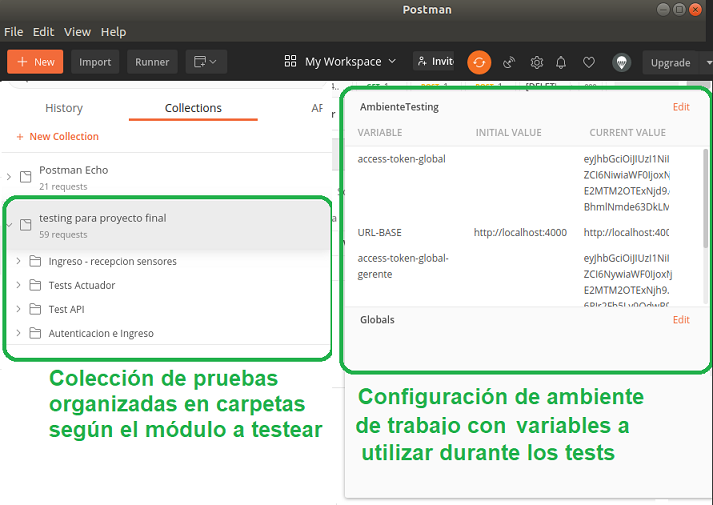
\includegraphics[width=1\textwidth]{./Figures/postman.png}
	\caption{Herramienta Postman junto a su configuración básica.}
	\label{fig:Postmanconfig}
\end{figure}

Por su parte, Newman permite importar los conjuntos de tests definidos en Postman, y mediante un script, ejecutar los mismos y ver los resultados obtenidos. De esta manera podemos correr todos los tests automáticamente, de forma rápida y simple, sin necesidad de hacerlo manualmente.

Para llevar adelante dicho procedimiento desde Postman se exportaron, tanto la colección de tests, como el ambiente de trabajo (\textit{environment} \citep{WEBSITE:EnvironmentPostman}). Esto generó dos archivos que se utilizaron para configurar la ejecución automática desde Newman. Luego, se desarrolló un script en el backend del trabajo para poder correr la colección con la herramienta de \textit{npm}.

En la figura \ref{fig:scriptNewman} se muestra el script generado y la configuración del mismo en el archivo package.json del módulo de backend.


\begin{figure}[ht]
	\centering
	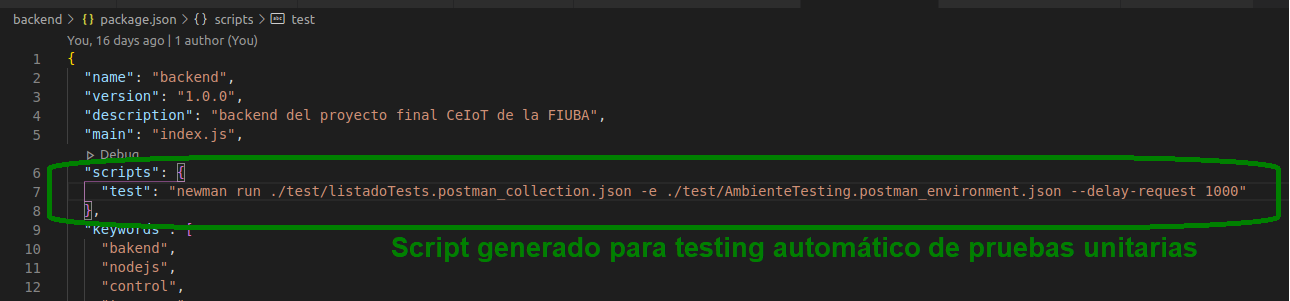
\includegraphics[width=1\textwidth]{./Figures/scriptNewman.png}
	\caption{Configuración del script para testing automático de pruebas unitarias.}
	\label{fig:scriptNewman}
\end{figure}

Por otra parte, en la figura \ref{fig:newmanEjecucion} se muestra la ejecución del script desde la consola de Visual Studio Code y los resultados obtenidos. 


\begin{figure}[ht]
	\centering
	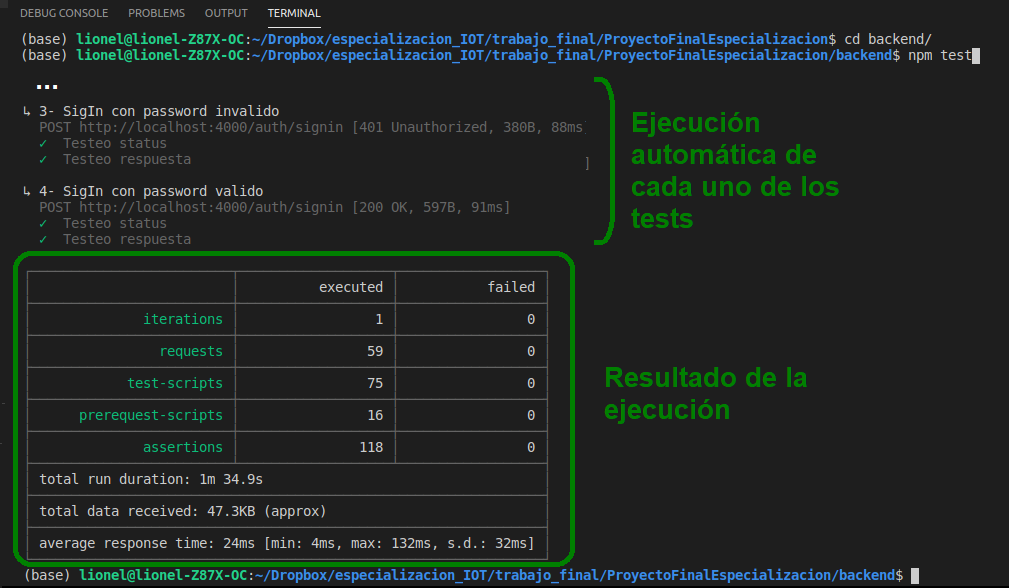
\includegraphics[width=1\textwidth]{./Figures/newmanEjecucion.png}
	\caption{Ejecución y resultados de ejecución del script automático de testing.}
	\label{fig:newmanEjecucion}
\end{figure}


\subsection{Mocks implementados}

Para aquellos módulos que tenían dependencias (interfaces) con otros se utilizaron \textit{mocks}, lo que posibilitó testearlos simulando el comportamiento de los dependientes, sin necesidad de tenerlos implementados.

Se desarrollaron dos \textit{mocks} en el trabajo:

\begin{enumerate}
\item mockActuador: permitió simular la operatoria del módulo actuador. El mismo se implementó como una aplicación web en Node.JS que respondía a las peticiones realizadas desde el backend.
\item mockSistemaTerceros: permitió simular la interfaz entre el sistema desarrollado y el sistema de documentación de terceros. El mismo se implementó como una aplicación web en Node.JS, 
\end{enumerate}
    
\clearpage
\section{Pruebas unitarias}

En esta sección se detalla el conjunto de pruebas unitarias realizadas sobre cada uno de los módulos del sistema.

\subsection{Testing del módulo sensor}

Al momento de testear el módulo sensor, ya se contaba con el módulo del backend desarrollado, con lo cual no fue necesario implementar un \textit{mock}.

Para proceder con las pruebas se configuraron algunas tarjetas RFID con diferentes valores que simularon cada uno de los escenarios posibles. Se utilizó con tal propósito un programa escrito en Arduino IDE que permitió asignar el valor a la tarjeta a través del monitor serie. Luego se alimentó el módulo y se procedió a testear cada caso, acercando una a una las tarjetas ya configuradas para observar los resultados obtenidos.

En la tabla \ref{tab:tablaTestNodSensor} se detalla el conjunto de casos de tests más relevantes implementados para probar el módulo sensor y sus resultados. \footnote{Para tener un detalle completo de los test remitirse al documento de Casos de Uso y Casos de Test \citep{WEBSITE:CasosUsoYTest}.}

\begin{table}[h]
	\centering
	\caption[Tipos de pruebas sensor]{Casos de test del módulo sensor.}
	\begin{tabular}{p{1.5cm} p{5.5cm} p{5.5cm}} 	

		\toprule
		\textbf{Caso test} & 
		\textbf{Escenario a testear} & 
		\textbf{Resultados} 
		\\
		\midrule
1 & Tarjeta RFID sin valor configurado. & El led ``PinTarjNoLeida'' se prende durante dos segundos y se apaga. \\
2 & Valor de tarjeta RFID recibido correctamente por el backend.	& El led ``PinOkSistema'' se prende durante dos segundos y se apaga. \\
3 & El módulo sensor no registrado en el sistema. & El led ``PinNoOkSistemaCodigo'' se prende durante dos segundos y se apaga. \\
4 & El módulo sensor no está activo en el sistema. & El led ``PinNoOkSistemaCodigo'' se prende durante dos segundos y se apaga. \\	   
		\bottomrule
		\hline
	\end{tabular}
	\label{tab:tablaTestNodSensor}
\end{table}

En la figura \ref{fig:TestTajetaSinCodigo} se muestra el caso de test 1 donde la tarjeta no tiene valor configurado. En la primera imagen se ve el momento en que se acerca la tarjeta y en la segunda imagen se ve el momento en que el módulo responde al usuario.

\begin{figure}[ht]
	\centering
	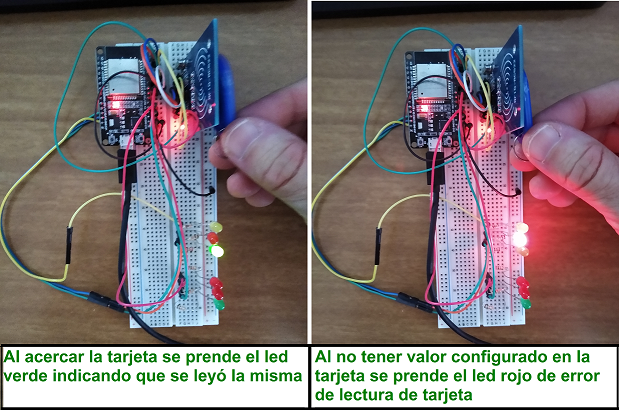
\includegraphics[width=0.8\textwidth]{./Figures/TestTajetaSinCodigo.png}
	\caption{Procedimiento de prueba para el caso de test 1 con tarjeta sin valor configurado.}
	\label{fig:TestTajetaSinCodigo}
\end{figure}


En la figura \ref{fig:TestTajetaCodigoLeida} se muestra el caso de test 2 donde la tarjeta es válida, y el sistema se comunica correctamente con el módulo del backend. En la primera imagen se ve el momento en que se acerca la tarjeta y en la segunda imagen se ve el momento en que el módulo responde al usuario.


\begin{figure}[ht]
	\centering
	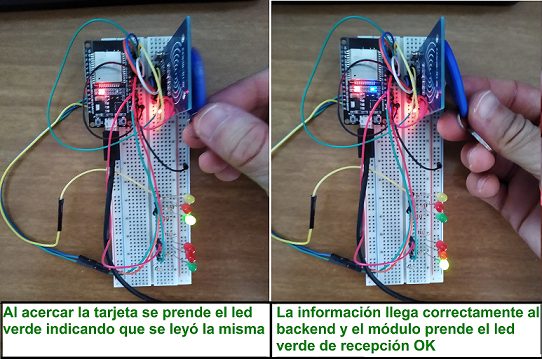
\includegraphics[width=0.8\textwidth]{./Figures/TestTajetaCodigoLeida.png}
	\caption{Procedimiento de prueba para el caso de test 2 con tarjeta con valor configurado y recibido correctamente por el backend.}
	\label{fig:TestTajetaCodigoLeida}
\end{figure}


\clearpage
\subsection{Testing del módulo actuador}

Para testear el módulo actuador se utilizó Postman, dado que el módulo expone una conexión HTTP POST. Dentro de Postman generamos una carpeta llamada Test Actuador, en la cual almacenamos todos los casos de test. En el \textit{body} se envían los valores como un objeto JSON.

En la figura \ref{fig:TestActuadorConfig} se muestra la configuración de Postman para el testeo del módulo actuador.

\begin{figure}[ht]
	\centering
	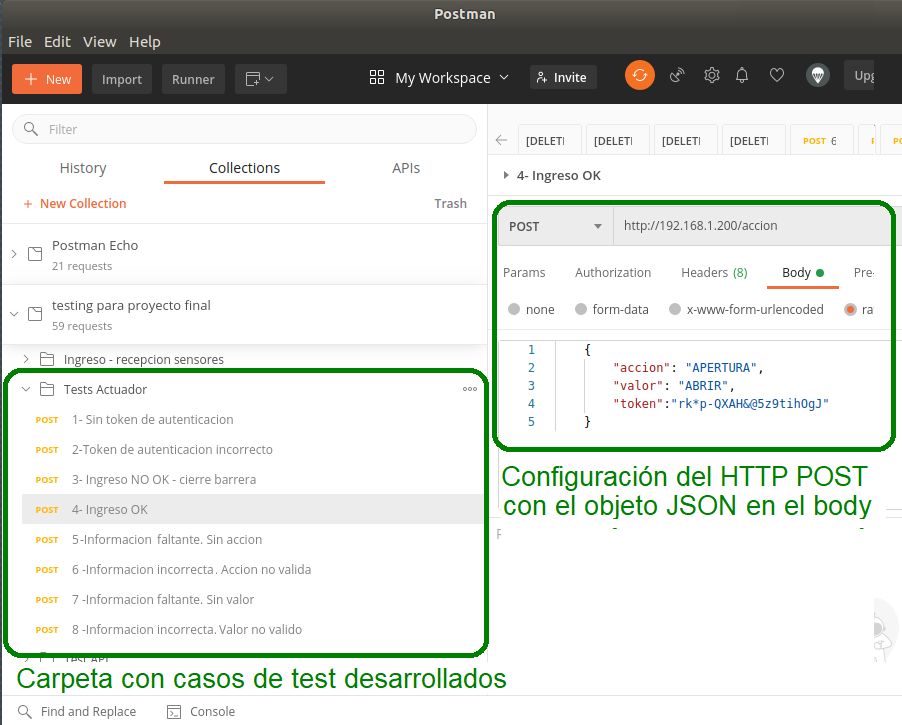
\includegraphics[width=0.9\textwidth]{./Figures/TestActuadorConfig.png}
	\caption{Configuración en Postman para el testeo del módulo actuador.}
	\label{fig:TestActuadorConfig}
\end{figure}

La prueba implicó testear cada uno de los casos generados, ejecutándolos desde Postman. A fin de automatizar los tests, y no depender de un control manual de la respuesta obtenida luego de cada ejecución, se configuraron para cada test las condiciones esperadas o aserciones, utilizando la sección ``Tests'' de la herramienta. Algunas de las aserciones definidas fueron que el código de estado HTTP sea el esperado y/o que la respuesta contenga cierto dato o cierto objeto JSON con determinados valores. Al ejecutar el test, si los resultados eran los previstos, Postman indicaba en el apartado ``Test Results'' que los mismos eran correctos.

En la figura \ref{fig:PostmanAsercion} se muestra un ejemplo de configuración de la sección ``Tests'' y la ejecución del caso de test.

\begin{figure}[ht]
	\centering
	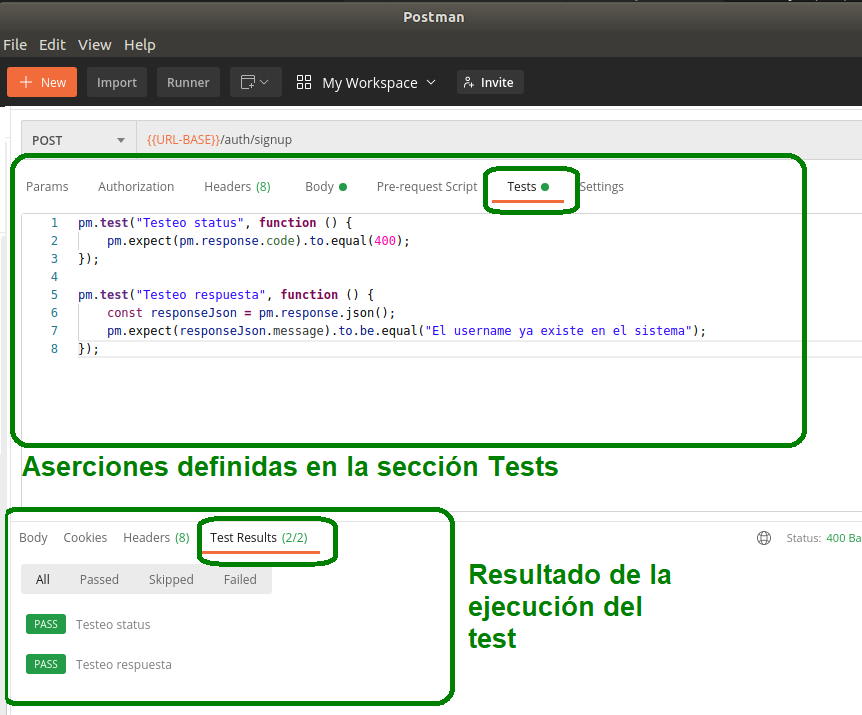
\includegraphics[width=1\textwidth]{./Figures/PostmanAsercion.png}
	\caption{Configuración de sección ``Tests'' y resultados de la ejecución del test.}
	\label{fig:PostmanAsercion}
\end{figure}

En la tabla  \ref{tab:tablaTestNodActuador} se detalla el conjunto de casos de tests más relevantes implementados para probar el módulo actuador y sus resultados. Dentro del escenario a testear entre paréntesis se hace referencia al nombre del test en Postman. \footnote{Para tener un detalle completo de los test remitirse al documento de Casos de Uso y Casos de Test \citep{WEBSITE:CasosUsoYTest}.}

\begin{table}[h]
	\centering
	\caption[Tipos de pruebas actuador]{Casos de test del módulo actuador.}
	\begin{tabular}{p{1.5cm} p{6.5cm} p{4.5cm}} 	

		\toprule
		\textbf{Caso test} & 
		\textbf{Escenario a testear} & 
		\textbf{Resultados} 
		\\
		\midrule
1 & Habilitar ingreso a la planta (Ingreso OK). & El led ``IngresoOk'' parpadea durante 4 segundos y se activa la cerradura. \\
2 & Inhabilitar ingreso a la planta (Ingreso NO OK – cierre barrera).	& El led ``IngresoNOOk'' se prende durante dos segundos y se apaga. \\
3 & El pedido HTTP POST no cuenta con el campo de acción a realizar (Información faltante – Acción no válida). & El led Error parpadea dos veces. \\
4 & El pedido HTTP POST no cuenta con token de autenticación (Sin token de autenticación). & El led Error parpadea una vez. \\	   
		\bottomrule
		\hline
	\end{tabular}
	\label{tab:tablaTestNodActuador}
\end{table}

En la sección \ref{sec:PruebasAceptacion} se muestra el detalle de los casos de ingreso habilitado e inhabilitado junto a una figura del módulo actuador. Remitirse a dicha sección para más detalles.

\pagebreak
\subsection{Testing del módulo de backend}

Para testear el módulo de backend se utilizó Postman, dado que el módulo expone una API Rest al frontend, una API de autenticación y un \textit{endpoint} \citep{WEBSITE:Endpoints} para recibir los datos de los módulos sensores. Dentro de Postman generamos una carpeta llamada ``Test API'' para testear la API expuesta al frontend, una carpeta llamada ``Autenticación e ingreso'' para testear la API de autenticación y una carpeta llamada ``Ingreso – recepción sensores'' para testear los ingresos generados desde el módulo sensor.

Dentro de la carpeta de ``Test API'' generamos cuatro subcarpetas para testear los casos sin autenticación y con autenticación para los diferentes perfiles de usuario. Dentro de la carpeta de ``Autenticación e ingreso'', se colocaron los tests para el alta de usuario y el ingreso al sistema. Y dentro de la capeta ``Ingreso – recepción sensores'', los tests para los ingresos generados desde el módulo sensor.

En la figura \ref{fig:testsBackend} se muestra las carpetas configuradas en Postman para el testeo de los casos de test de backend.

\begin{figure}[h]
	\centering
	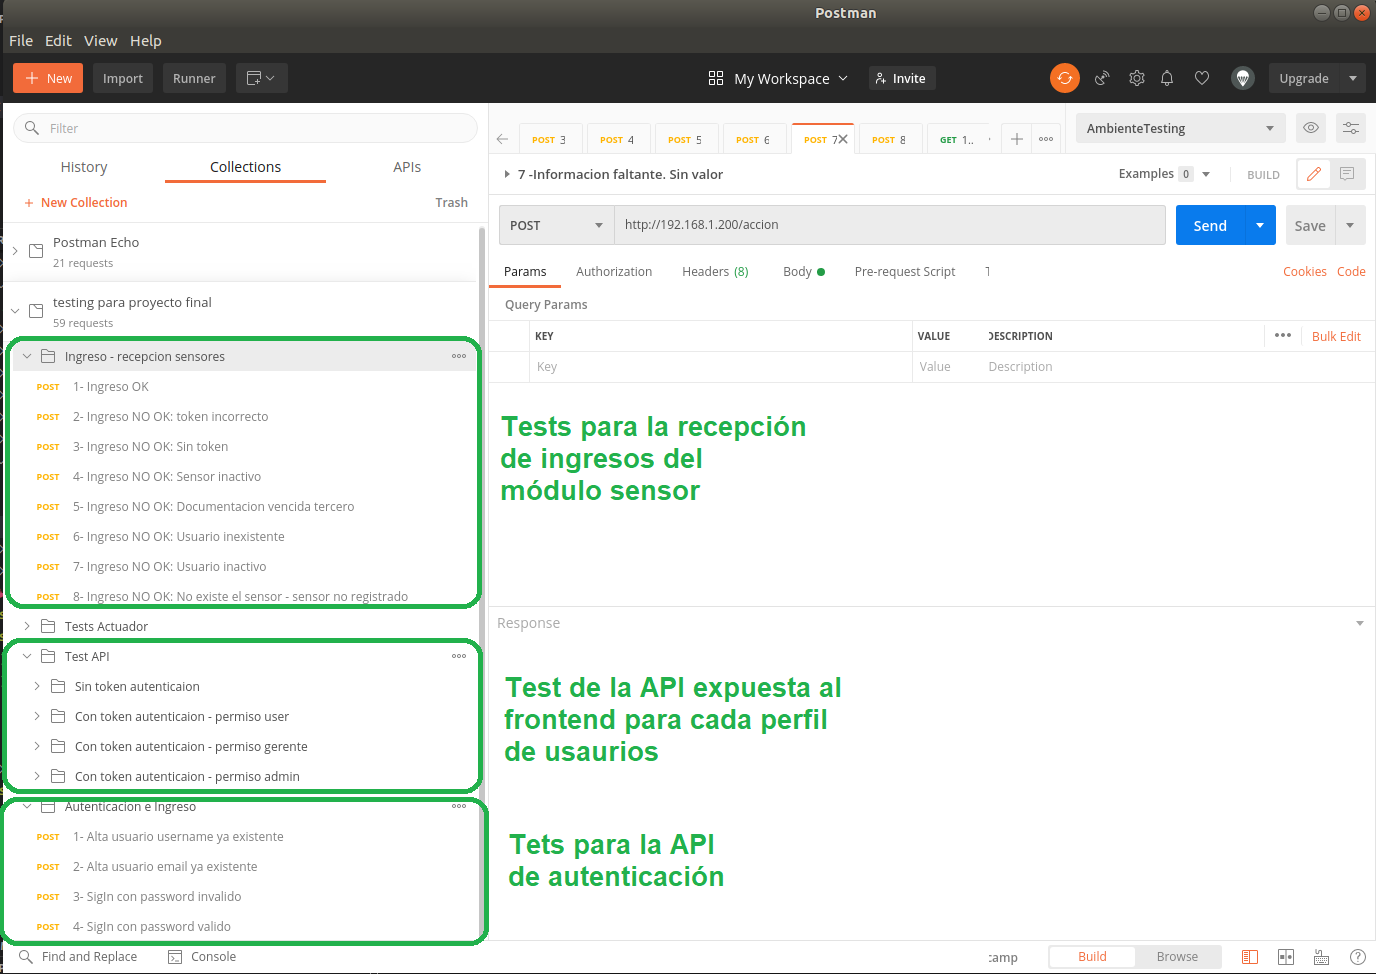
\includegraphics[width=1\textwidth]{./Figures/testsBackend.png}
	\caption{Configuración en Postman para el testeo del módulo de backend.}
	\label{fig:testsBackend}
\end{figure}


Para testear cada caso, se procedió a configurar en Postman la URL de cada \textit{endpoint}, junto a los parámetros requeridos. Para los pedidos HTTP GET se configuró directamente la URL con los parámetros, y para los HTTP POST se completó el \textit{body} con el objeto JSON, junto a los valores requeridos según cada caso. 

\pagebreak
Para los casos de test con autenticación definidos dentro de la carpeta ``Test API'', se procedió a utilizar los \textit{environments} y las variables globales de Postman. Un \textit{environment} permite definir ambientes de testing dentro de los cuales podemos definir variables globales que pueden utilizarse en varios tests. Un test puede obtener un valor de la respuesta HTTP y guardarlo en una variable global para luego ser utilizado por otro. De este modo, definimos un \textit{environment} llamado ``AmbienteTesting'' y dentro del mismo configuramos las siguientes variables globales:

\begin{itemize}
\item URL-BASE: contiene la URL base del backend a partir del cual se define cada \textit{endpoint}. Con la misma configuramos cada HTTP POST o GET, de modo que si cambia la URL de nuestro backend, con solo modificar esta variable quedan ajustados todos los \textit{endpoints}.

\item Access-token-global: utilizado para los \textit{endpoints} que son accesibles para cualquier usuario del sistema. Permite guardar el token de acceso del rol usuario.

\item Access-token-global-gerente: utilizado para los \textit{endpoints} que son accesibles solo por el perfil de gerente de la aplicación. Permite guardar el token de acceso del rol gerente.

\item Access-token-global-admin: utilizado para los \textit{endpoints} que son accesibles solo por el perfil de administrador de la aplicación. Permite guardar el token de acceso para el rol de administrador.
\end{itemize}

Los tokens de acceso se configuran dentro de la sección header del test, con clave x-access-token y con el valor del token.

En la figura \ref{fig:PostmanEnvironmnet} se muestran las variables globales definidas en Postman.

\begin{figure}[ht]
	\centering
	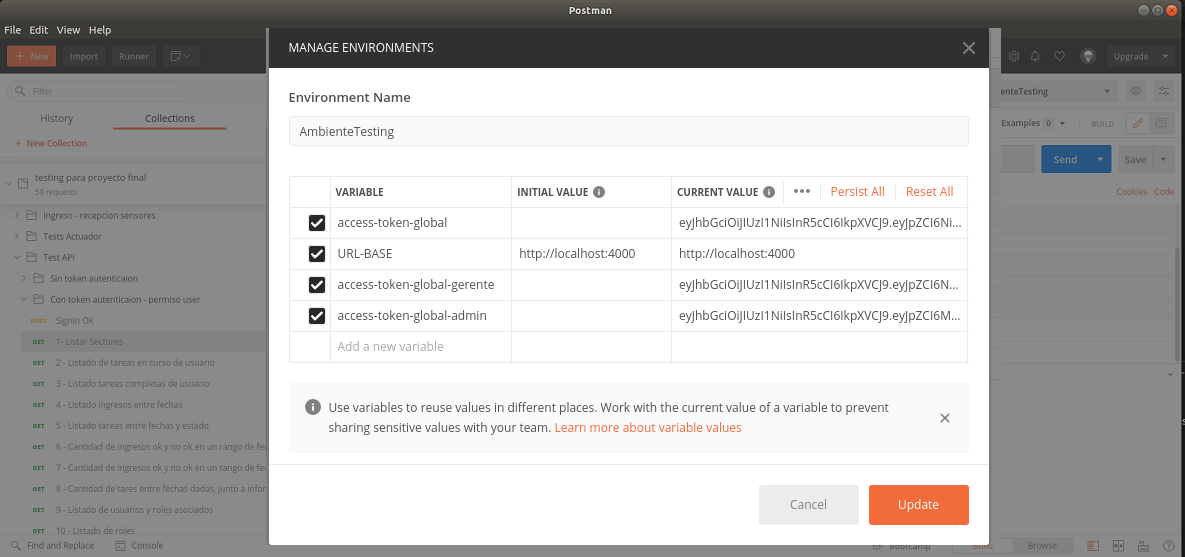
\includegraphics[width=1\textwidth]{./Figures/PostmanEnvironmnet.png}
	\caption{Variables globales definidas en Postman.}
	\label{fig:PostmanEnvironmnet}
\end{figure}

\subsubsection{Tests de la carpeta Test API }

Dentro de la carpeta Test API tenemos cuatro subcarpetas:

\begin{itemize}
\item Sin token autenticación: testea los \textit{endpoints} sin un token de autenticación.
\item Con token autenticación – permiso user: testea los \textit{endpoints}  que son accesibles para cualquier usuario del sistema. En esta carpeta se define un test inicial llamado ``SigIn OK'', que se utilizó para simular la autenticación de un usuario normal y completar la variable global access-token-global que fue utilizada por el resto de los tests de la carpeta.
\item Con token autenticación – permiso gerente: testea los \textit{endpoints}  que son accesibles para el usuario con rol gerente. En esta carpeta se define un test inicial llamado ``SigIn OK'', que se utilizó para simular la autenticación de un usuario gerente y completar la variable global access-token-global-gerente que fue utilizada por el resto de los tests de la carpeta.
\item Con token autenticación – permiso admin: testea los \textit{endpoints} que son accesibles para el usuario con rol administrador. En esta carpeta se define un test inicial llamado ``SigIn OK'', que se utilizó para simular la autenticación de un usuario administrador y completar la variable global access-token-global-admin que fue utilizada por el resto de los tests de la carpeta.
\end{itemize}

En la figura \ref{fig:TestBackendGerente} se muestran los tests de la subcarpeta ``Con token autenticación – permiso gerente'', junto al test inicial ``SignIn OK'' y al resto de los tests.

\begin{figure}[ht]
	\centering
	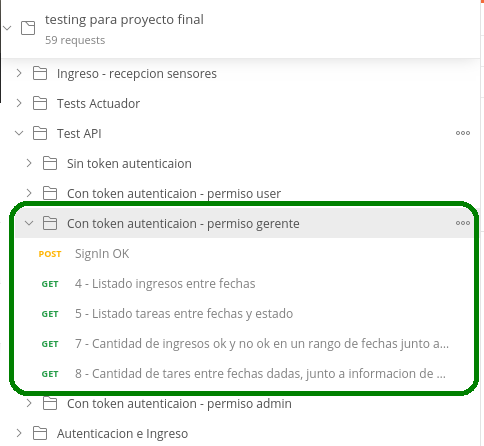
\includegraphics[width=0.7\textwidth]{./Figures/TestBackendGerente.png}
	\caption{Tests de la subcarpeta Con token autenticación – permiso gerente.}
	\label{fig:TestBackendGerente}
\end{figure}

\pagebreak
\subsubsection{Detalle de tests y resultados}

En la tabla  \ref{tab:tablaTestBackendSensor} se detalla el conjunto de casos de tests más relevantes implementados para probar la recepción de los datos de los módulos sensores y sus resultados. En la columna escenario a testear se hace referencia, entre paréntesis, al número del test en Postman.  \footnote{Para tener un detalle completo de los test remitirse al documento de Casos de Uso y Casos de Test \citep{WEBSITE:CasosUsoYTest}.}


\begin{table}[h]
	\centering
	\caption[Tipos de pruebas backend]{Casos de test del módulo backend. Testing de recepción de los datos de los módulos sensores.}
	\begin{tabular}{p{3.5cm} p{4.5cm} p{4cm}} 	

		\toprule
		\textbf{Subcarpeta Postman} & 
		\textbf{Escenario a testear} &
		\textbf{Resultados} 
		\\
		\midrule

 Ingreso – recepción sensores.                  
& Ingreso con valor de tarjeta registrado en el sistema y módulo sensor activo (1).
& Se confirma recepción con HTTP código 200.  \\
& El módulo sensor no está registrado en el sistema  (8).
& Se rechaza el ingreso con mensaje de error de sensor inexistente. \\
& El módulo sensor no está activo en el sistema (4). 
& Se rechaza el ingreso con mensaje de error de sensor inactivo. \\
		\bottomrule
		\hline
	\end{tabular}
	\label{tab:tablaTestBackendSensor}
\end{table}

En la tabla  \ref{tab:tablaTestBackendAutenticacion} se detalla el conjunto de casos de tests más relevantes implementados para probar la API de autenticación y sus resultados. En la columna escenario a testear se hace referencia, entre paréntesis, al número del test en Postman.

\begin{table}[h]
	\centering
	\caption[Tipos de pruebas backend]{Casos de test del módulo backend. Testing de la API de autenticación.}
	\begin{tabular}{p{3.5cm} p{4.5cm} p{4cm}} 	

		\toprule
		\textbf{Subcarpeta Postman} & 
		\textbf{Escenario a testear} &
		\textbf{Resultados} 
		\\
		\midrule
\multirow{3}{3.5cm}{Autenticación e ingreso.} & Alta de usuario con username, email y password correcto (5). & Se confirma el alta del usuario con HTTP código 200. \\
                    & Alta de usuario con username o email repetido (1 y2). & Se rechaza el alta. Respuesta HTTP con código 400 y mensaje de error. \\
                    & Inicio de sesión con username o password incorrecto (3 y 4). & Se rechaza el inicio de sesión. Respuesta HTTP con código 401 y mensaje de error. \\
		\bottomrule
		\hline
	\end{tabular}
	\label{tab:tablaTestBackendAutenticacion}
\end{table}

En la tabla \ref{tab:tablaTestBackendFrontend} se detalla el conjunto de casos de tests más relevantes implementados para probar la API Rest expuesta al frontend y sus resultados. En la columna escenario a testear se hace referencia, entre paréntesis, al número del test en Postman.  \footnote{\label{notaReusadaCasosTest}Para tener un detalle completo de los test remitirse al documento de Casos de Uso y Casos de Test \citep{WEBSITE:CasosUsoYTest}.}


\begin{table}[h]
	\centering
	\caption[Tipos de pruebas backend]{Casos de test del módulo backend. Testing de la API Rest expuesta al frontend.}
	\begin{tabular}{p{3.5cm} p{3.5cm} p{5cm}} 	

		\toprule
		\textbf{Subcarpeta Postman} & 
		\textbf{Escenario a testear} &
		\textbf{Resultados} 
		\\
		\midrule

\multirow{2}{3.5cm}{Test API/Sin token autenticación.} & Listar sectores de la empresa (1). & Se acepta el pedido y se devuelve el listado de sectores de la empresa. \\
                    & Resto de los \textit{endpoints}. & Se rechaza el pedido por falta de token de autenticación con un HTTP 403. \\
\hline
\multirow{3}{3.5cm}{Test API/Con token autenticación – permiso user.} & Listado de tareas en curso del usuario (2). & Se acepta el pedido y se devuelve el listado de tareas en curso del usuario. \\
                    & Listado de tareas completas del usuario (3). & Se acepta el pedido y se devuelve el listado de tareas completas del usuario. \\
                    & Cantidad ingresos a la empresa por día (7). & Se rechaza el pedido por no tener rol gerente o administrador con un HTTP 403. \\
\hline
\multirow{2}{3.5cm}{Test API/Con token autenticación – permiso gerente.}  & Cantidad ingresos a la empresa por día (7). & Se acepta el pedido y se devuelve el listado de ingresos OK y no OK para las fechas indicadas. \\
                    & Listado detalle de tareas en curso entre rango de fechas (5). & Se acepta el pedido y se devuelve el listado de tareas y sub-tareas para las fechas indicadas. \\
\hline
\multirow{2}{3.5cm}{Test API/Con token autenticación – permiso admin.}  & Listado de usuarios y roles (9). & Se acepta el pedido y se devuelve el listado de usuarios y roles de cada usuario. \\
                    & Cambiar estado de rol de usuario (12). & Se acepta el pedido y ajusta el estado del rol para el usuario indicado. \\
		\bottomrule
		\hline
	\end{tabular}
	\label{tab:tablaTestBackendFrontend}
\end{table}

\pagebreak
\section{Pruebas de sistema}

En esta sección se detalla el conjunto de pruebas integrales realizadas sobre el sistema con todos sus módulos. Este test fue ejecutado por el desarrollador en el ambiente de pruebas, sin el cliente.

Una vez implementados todos los módulos, se realizaron las siguientes tareas:

\begin{enumerate}
\item Se crearon usuarios con cada uno de los roles en la base de datos.
\item Se alimentó el módulo sensor y el módulo actuador.
\item Se corrió el módulo de backend, el \textit{mock} del sistema de terceros y el módulo de frontend. Con el propósito de automatizar este paso, se desarrolló un script para ejecutar y levantar los módulos antes mencionados, mediante el uso de contenedores \textit{Docker} y de la herramienta \textit{docker-compose}. 

\end{enumerate}

Con los módulos en ejecución, se procedió a \textit{loguearse} en la aplicación. En primer lugar, con un rol de usuario normal, luego con el rol de usuario gerente, posteriormente con el rol vigilante y por último con el rol administrador.

En la tabla  \ref{tab:tablaTestsSistemaUsuNormal} se detalla el conjunto de casos de tests más relevantes implementados para probar el rol de usuario normal (rol user) y los resultados obtenidos.\footnote{\label{notaReusadaCasosTest}Para tener un detalle completo de los test remitirse al documento de Casos de Uso y Casos de Test \citep{WEBSITE:CasosUsoYTest}.}

\begin{table}[h]
	\centering
	\caption[Tipos de pruebas sistema]{Listado de pruebas realizadas para el rol de usuario normal.}
	\begin{tabular}{ p{3.5cm} p{2.5cm} p{7cm}}

		\toprule
		\textbf{Pantalla del sistema testeada} & 
		\textbf{Acción} & 
		\textbf{Resultados} 
		\\
		\midrule
Mis tareas en curso  & Visualizar tareas.  & Se muestra el listado de tareas en curso del usuario o se indica que no tiene tareas en curso. \\
Mis tareas en curso & Cerrar tarea.  & Se marca como completa la tarea del usuario y se muestra una alerta indicando que se cerró la tarea correctamente.  \\
Mis tareas en curso & Ajustar observación en tarea.  & Se ajusta la observación en la tarea y se muestra una alerta indicando que se actualizó la observación correctamente. \\
Mi historial tareas & Visualizar historial tareas de usuario. & Se muestra el listado de tareas cerradas del usuario o se indica que no tiene tareas cerradas. \\
Mi perfil & Visualizar perfil. & Se muestra la información del usuario, incluyendo su \textit{username}, email, sector y roles asignados. \\

		\bottomrule
		\hline
	\end{tabular}
	\label{tab:tablaTestsSistemaUsuNormal}
\end{table}


En la tabla  \ref{tab:tablaTestsSistemaUsuAdmin} se detalla el conjunto de casos de tests más relevantes implementados para probar el rol de usuario administrador y los resultados obtenidos. 

\begin{table}[h]
	\centering
	\caption[Tipos de pruebas sistema]{Listado de pruebas realizadas para el rol de usuario administrador.}
	\begin{tabular}{ p{3.5cm} p{2.5cm} p{7cm}} 	

		\toprule
		\textbf{Pantalla del sistema testeada} & 
		\textbf{Acción} & 
		\textbf{Resultados} 
		\\
		\midrule
Gestión usuarios & Modificar estado de rol de usuario.  & Se modifica el estado del rol del usuario en la base de datos y se muestra una alerta indicando que el cambio se realizó correctamente.  \\
		\bottomrule
		\hline
	\end{tabular}
	\label{tab:tablaTestsSistemaUsuAdmin}
\end{table}

En la tabla  \ref{tab:tablaTestsSistemaUsuGerente} se detalla el conjunto de casos de tests más relevantes implementados para probar el rol de usuario gerente y los resultados obtenidos. 

\begin{table}[h]
	\centering
	\caption[Tipos de pruebas sistema]{Listado de pruebas realizadas para el rol de usuario gerente.}
	\begin{tabular}{p{3.5cm} p{2.5cm} p{7cm}}

		\toprule
		\textbf{Pantalla del sistema testeada} & 
		\textbf{Acción} & 
		\textbf{Resultados} 
		\\
		\midrule
Estadísticas ingresos & Visualizar ingresos del mes.  & Se muestra un gráfico de barras con la cantidad de ingresos de cada día del mes especificado (ingresos ok y no ok) y un gráfico de torta con el total de ingresos ok y no ok del mes.  \\
Estadísticas tareas & Visualizar estadísticas de tareas.  & Se muestra un gráfico de torta con la cantidad de tareas en curso, un gráfico de barras con la cantidad de tareas cerradas por cada mes del año y un gráfico de torta con el total de tareas completas del año.  \\
Tareas en curso & Visualizar tareas en curso.
  & Se muestra el listado de tareas en curso, junto a información de antigüedad, estado, fecha de inicio y detalle de las sub-tarea de cada sector.  \\
Ingresos del día & Visualizar ingresos del día.  & Se muestra el listado de los ingresos, junto a información de horario, si el ingreso fue permitido o no y el detalle de la habilitación o rechazo junto al nombre del tercero.  \\

		\bottomrule
		\hline
	\end{tabular}
	\label{tab:tablaTestsSistemaUsuGerente}
\end{table}

En la tabla  \ref{tab:tablaTestsSistemaUsuPorteria} se detalla el conjunto de casos de tests más relevantes implementados para probar el rol de usuario vigilante y los resultados obtenidos. 

\begin{table}[h]
	\centering
	\caption[Tipos de pruebas sistema]{Listado de pruebas realizadas para el rol de usuario vigilante.}
	\begin{tabular}{p{3.5cm} p{2.5cm} p{7cm}}

		\toprule
		\textbf{Pantalla del sistema testeada} & 
		\textbf{Acción} & 
		\textbf{Resultados} 
		\\
		\midrule
Pantalla principal & Visualizar ingreso en portería.  & Cuando un tercero pretende ingresar en planta, se muestra en la pantalla principal una alerta, indicando el intento de acceso y si el mismo se permitió o se rechazó, junto a un color particular para diferenciar ambos casos. La alerta se muestra por 6 segundos. \\
		\bottomrule
		\hline
	\end{tabular}
	\label{tab:tablaTestsSistemaUsuPorteria}
\end{table}


\pagebreak
\section{Pruebas de aceptación}\label{sec:PruebasAceptacion}

En esta sección se detallan dos de las pruebas de aceptación realizadas en conjunto con el cliente. Estos tests fueron llevados a cabo por el desarrollador, en el ambiente de pruebas, para verificar el funcionamiento correcto del sistema implementado.

Para preparar dicho ambiente se procedió de igual modo que el descripto en la sección anterior para las pruebas de sistema.

\subsection{Descripción y detalles de prueba de ingreso habilitado}

En esta sección se detalla la prueba de ingreso de un tercero a la empresa que cuenta con la documentación requerida en regla.

Para realizar la prueba se preparó el sistema y se lo dejó operativo. Se utilizó la tarjeta RFID de un tercero que estaba habilitado y un usuario con rol de vigilancia generado previamente.

A continuación, se detallan los pasos realizados para el caso descripto:

\begin{enumerate}
\item Se ingresó a la aplicación con el usuario Portería y se accedió a la página principal.
\item Se tomó la tarjeta RFID del personal de tercero habilitado y se la acercó al módulo sensor. Como respuesta a esta interacción, sucedieron las siguientes acciones:

	\begin{enumerate}
	\item El módulo sensor prendió el led verde de lectura de la tarjeta y luego prendió el led verde de comunicación correcta con el backend.
	\item En la pantalla del usuario de portería se visualizó la alerta de ingreso del tercero durante 6 segundos. A continuación, se corroboró que el contador de ingresos correctos se había incrementado en la pantalla.
	\item El módulo actuador prendió de forma intermitente el led verde de ingreso habilitado durante 4 segundos y se cerró el pestillo de la cerradura electrónica. Pasado ese tiempo el pestillo se abrió nuevamente.
	\end{enumerate}


\end{enumerate}

En la figura \ref{fig:TestTajetaCodigoLeida2} se muestra el paso 2 de la prueba con el acercamiento de la tarjeta RFID al módulo sensor y la respuesta de dicho módulo.

\vspace{1cm}
\begin{figure}[h]
	\centering
	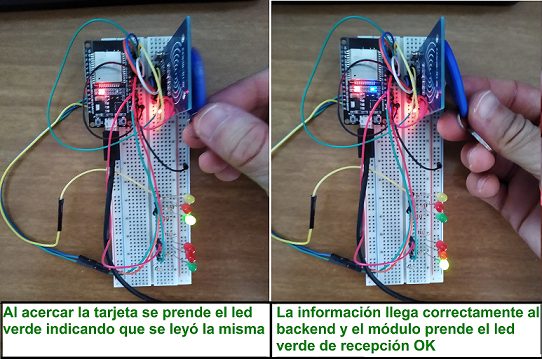
\includegraphics[width=1\textwidth]{./Figures/TestTajetaCodigoLeida.png}
	\caption{Accionamiento de módulo sensor con tarjeta RFID y respuesta del módulo.}
	\label{fig:TestTajetaCodigoLeida2}
\end{figure}

En la figura \ref{fig:ingresoOk} se muestra el paso 2 b) de prueba con la información visualizada por la vigilancia.

\begin{figure}[h]
	\centering
	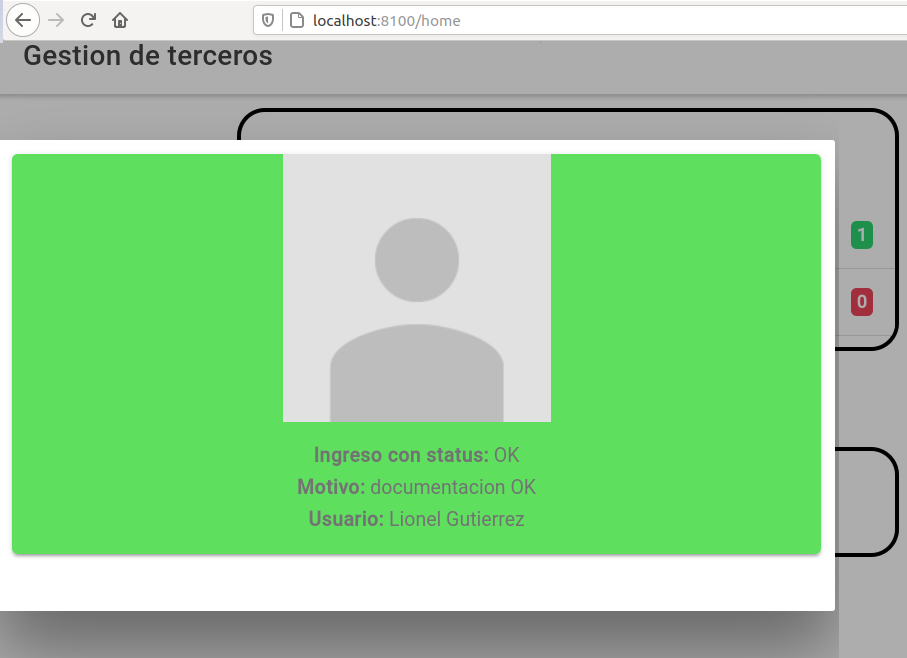
\includegraphics[width=1\textwidth]{./Figures/ingresoOk.png}
	\caption{Visualización de la alerta recibida en pantalla.}
	\label{fig:ingresoOk}
\end{figure}

En la figura \ref{fig:actuadorOK} se muestra el paso 2 c) de la prueba, donde se ve el módulo actuador con el led prendido y el pestillo de la cerradura cerrada.

\begin{figure}[h]
	\centering
	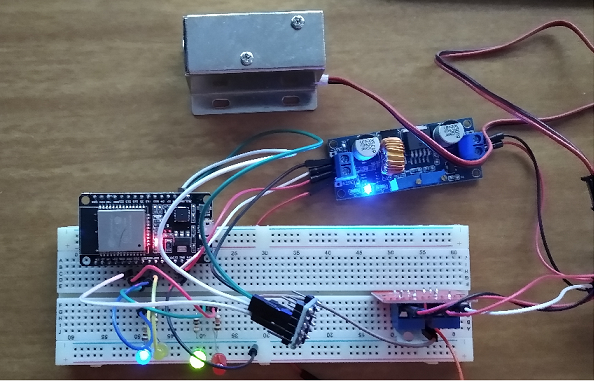
\includegraphics[width=1\textwidth]{./Figures/actuadorOK.png}
	\caption{Accionamiento de módulo actuador y respuesta del módulo.}
	\label{fig:actuadorOK}
\end{figure}

\clearpage
\subsection{Descripción y detalles de prueba de ingreso inhabilitado}

En esta sección se detalla la prueba de ingreso de un tercero a la empresa que no cuenta con la documentación requerida en regla.

Para realizar la prueba se preparó el sistema y se lo dejó operativo. Se utilizó la tarjeta RFID de un tercero que tenía problemas con su documentación y un usuario con rol de vigilancia generado previamente.

A continuación, se detallan los pasos realizados para el caso descripto:

\begin{enumerate}
\item Se ingresó a la aplicación con el usuario Portería y se accedió a la página principal.
\item Se tomó la tarjeta RFID del personal de tercero inhabilitado y se acercó la misma al módulo sensor. Como respuesta a esta interacción, sucedieron las siguientes acciones:

	\begin{enumerate}
	\item El módulo sensor prendió el led verde de lectura de la tarjeta y luego prendió el led verde de comunicación correcta con el backend.
	\item En la pantalla del usuario de portería se visualizó la alerta de ingreso inhabilitado del tercero durante 6 segundos. A continuación, se corroboró que el contador de intento de ingresos incorrectos se había incrementado en la pantalla.
	\item El módulo actuador prendió durante 2 segundos el led rojo de ingreso inhabilitado. El pestillo de la cerradura electrónica se mantuvo abierto todo el tiempo.
	\item Se envió un email a los usuarios de los sectores encargados de controlar la documentación del tercero, con el detalle del intento de ingreso.
	\item Se generó una tarea de control de documentación para cada uno de los sectores de la empresa responsables del proceso.
	\end{enumerate}

\item Se ingresó a la aplicación con un usuario de sector HESA (Seguridad y Medio Ambiente) para corroborar la generación de la tarea de control. Se accedió a la aplicación ``Mis tareas en curso'' y se visualizó la nueva tarea asignada al usuario.
\end{enumerate}

En la figura \ref{fig:ingresNOOK} se muestra el paso 2 b) de la prueba con la información visualizada por la vigilancia.

\begin{figure}[ht]
	\centering
	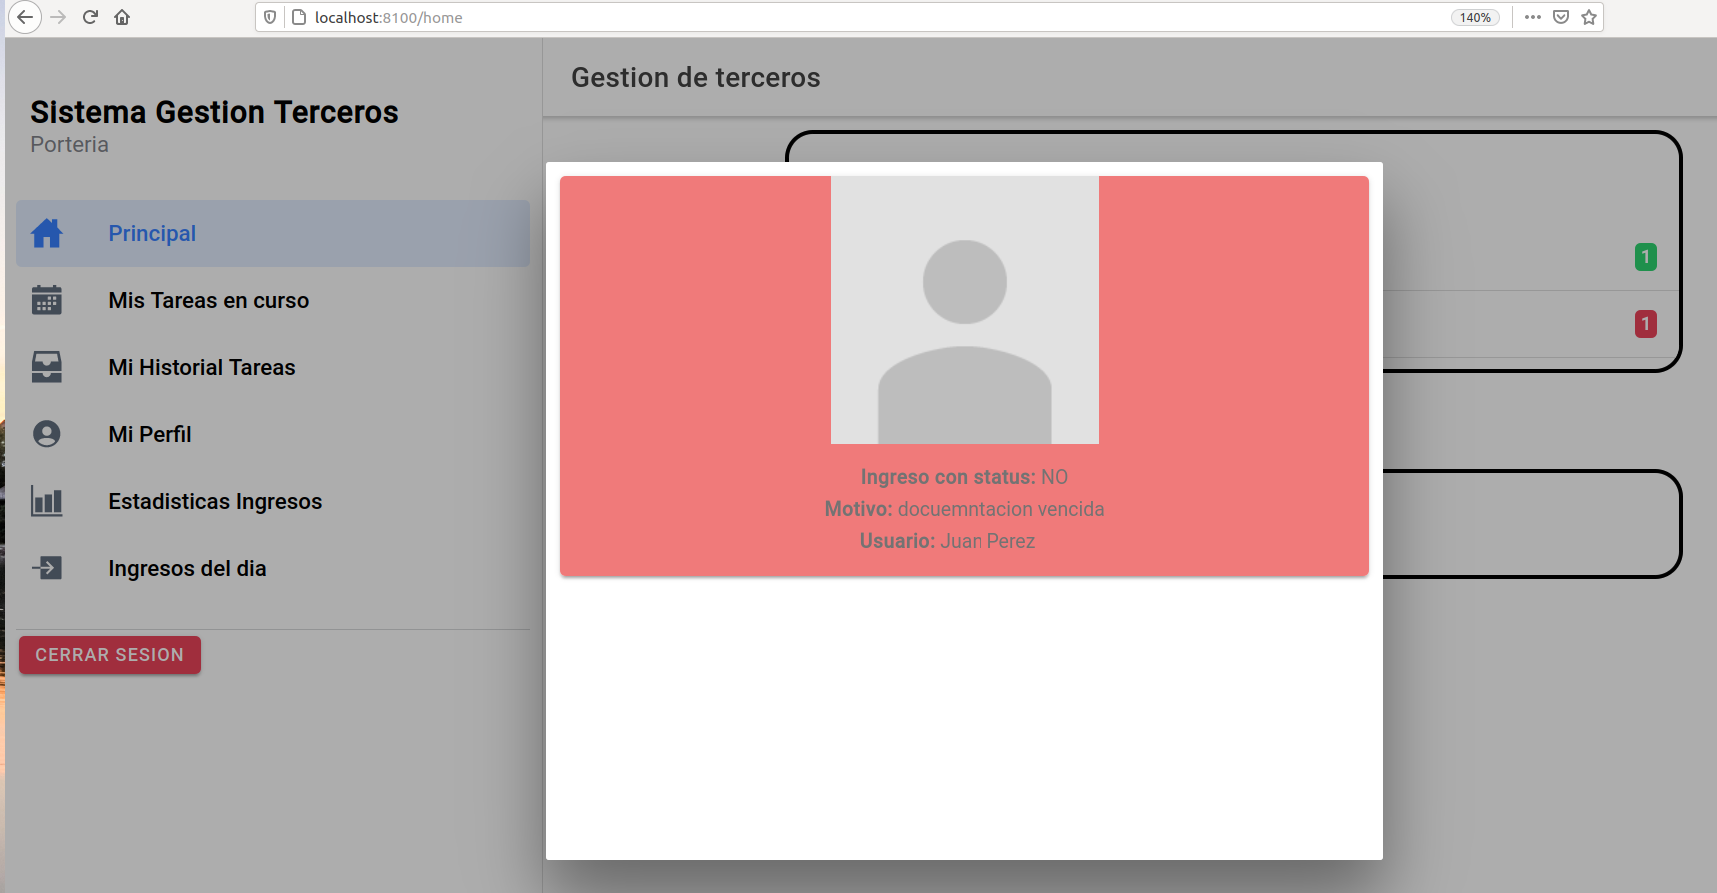
\includegraphics[width=1\textwidth]{./Figures/ingresoNOOK.png}
	\caption{Visualización de la alerta recibida en pantalla.}
	\label{fig:ingresNOOK}
\end{figure}

En la figura \ref{fig:actuadorNOOK} se muestra el paso 2 c) de la prueba, donde se ve el módulo actuador con el led rojo prendido y el pestillo de la cerradura abierta.

\begin{figure}[ht]
	\centering
	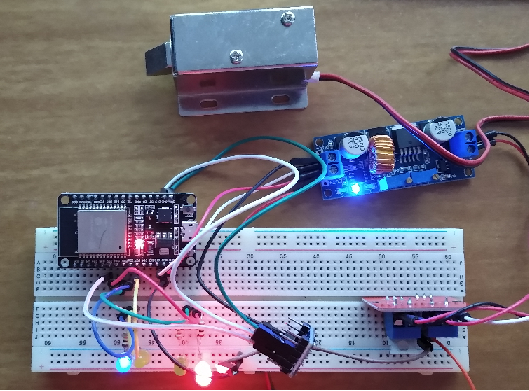
\includegraphics[width=1\textwidth]{./Figures/actuadorNOOK.png}
	\caption{Accionamiento de módulo actuador y respuesta del módulo.}
	\label{fig:actuadorNOOK}
\end{figure}

\clearpage
En la figura \ref{fig:Email} se ve el paso 2 d) de la prueba, con el email recibido por el usuario con la alerta del intento de ingreso con documentación vencida.

\begin{figure}[ht]
	\centering
	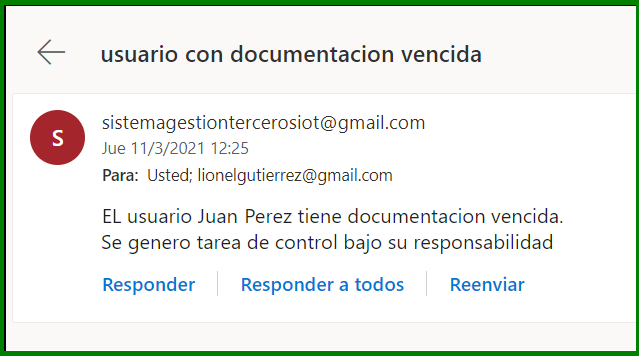
\includegraphics[width=1\textwidth]{./Figures/email.png}
	\caption{Email recibido por el usuario con la alerta de intento de ingreso con documentación vencida.}
	\label{fig:Email}
\end{figure}

En la figura \ref{fig:Tarea} se ve el paso 3 de la prueba, donde el usuario ve la tarea generada por parte del usuario.

\begin{figure}[ht]
	\centering
	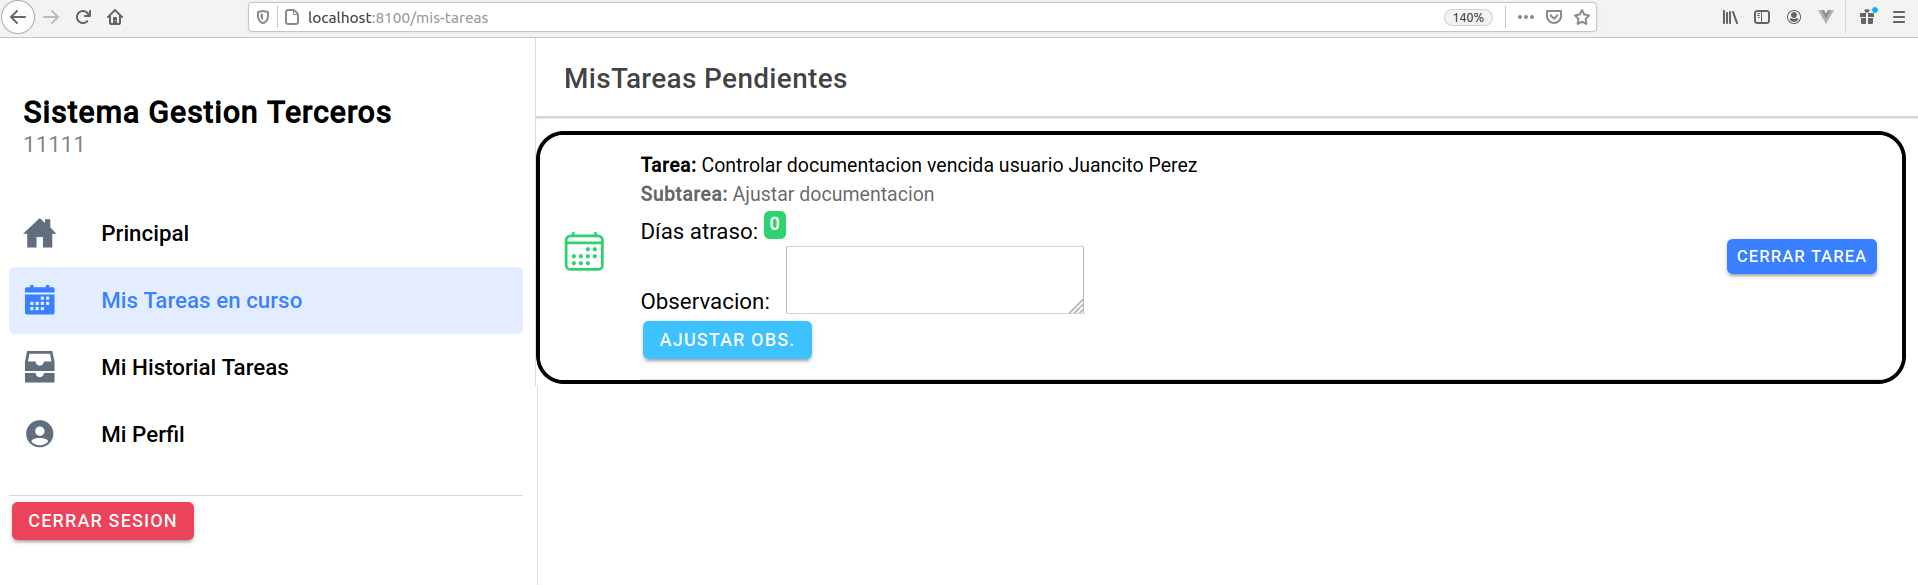
\includegraphics[width=1\textwidth]{./Figures/tarea.png}
	\caption{Pantalla de usuario se sector HESA con la tarea de control generada.}
	\label{fig:Tarea}
\end{figure}

\clearpage
\section{Comparativa con otras soluciones del mercado}\label{sec:comparativa}

A modo de conclusión de los ensayos realizados, se hace una comparativa contra soluciones similares que existen en el mercado para el control de ingreso. De acuerdo con el análisis comparativo realizado, se destaca el diferencial de este sistema al permitir comunicarse con otros sistemas de terceros y lograr una gestión integral de accesos, con capacidad de generar alertas y tareas de control sobre el proceso.

En la tabla \ref{tab:comparacionfinal} se muestra la comparación entre el sistema implementado y soluciones similares del mercado, en la que se puede apreciar el diferencial del sistema desarrollado.


\begin{table}[h]
	\centering
	\caption[Comparación soluciones]{Comparación contra otras soluciones similares del mercado.}
	\begin{tabular}{l c c c}   
		\toprule
		\textbf{Característica} & 
		\textbf{Sistema } & 
		\textbf{Pronext KY800} &	
		\textbf{Samsung H505}    
		\\
		\midrule
		Log de ingresos  & Si  & Si & No \\		
		Interfaz a sistemas externos & Si & No & No \\		
		Gestión integral de accesos & Si & No & No \\		
		Máximo usuarios & Indefinido & 500  & 30  \\		
		Conectividad/Protocolos & Wi-Fi & Bluetooth & No  \\		
		Doble factor autenticación & No  & No & Si \\
		Tarjetas RFID  & Si  & Si  & Si \\
		Alerta de acceso  & Si & Si & Si \\
		Acceso con huella & No & Si & No \\
		\bottomrule
		\hline
	\end{tabular}
	\label{tab:comparacionfinal}
\end{table}